\documentclass[12pt,a4paper]{article}
\usepackage[utf8]{inputenc}
\usepackage[spanish]{babel}
\usepackage{graphicx}
\usepackage{booktabs}
\usepackage{tabularx}
\usepackage{float}
\usepackage[hidelinks]{hyperref}
\usepackage{geometry}
\usepackage{fancyhdr}
\usepackage{tcolorbox}
\usepackage{enumitem}
\usepackage{amsmath}
\usepackage{listings}
\usepackage{xcolor}
\geometry{top=2.5cm, bottom=2.5cm, left=3cm, right=3cm}

\pagestyle{fancy}
\fancyhf{}
\rhead{Aseguramiento de la Calidad del Software -- NRC 30733}
\lhead{Grupo 7 -- Calidad en Uso}
\cfoot{\thepage}

\lstset{
    basicstyle=\ttfamily\small,
    backgroundcolor=\color{gray!10},
    frame=single,
    breaklines=true,
    language=Python,
    keywordstyle=\color{blue!80!black},
    commentstyle=\color{green!60!black},
    stringstyle=\color{red!60!black},
}

\begin{document}

% ============================================================
% CARATULA
% ============================================================
\begin{titlepage}
\centering
{\Large \textbf{Departamento de Ciencias de la Computaci\'on}}\\[0.3cm]
{\large Ingenier\'ia de Software}\\[1.5cm]

{\LARGE \textbf{Escenario 7: Obtenci\'on y Validaci\'on\\de Datos}}\\[0.5cm]
{\large Medici\'on de la Calidad en Uso mediante ISO/IEC 25022}\\[0.3cm]
{\large Caso de estudio: Red Hospitalaria MediSalud Ecuador}\\[2cm]

\begin{tabular}{ll}
\textbf{Asignatura:} & Aseguramiento de la Calidad del Software \\
\textbf{NRC:}        & 30733 \\
\textbf{Docente:}    & Ing. Diego Gamboa \\
\textbf{Repositorio:} & \url{https://github.com/kfamaguana07/medisalud-calidad-uso.git} \\
\end{tabular}\\[1.5cm]

\textbf{Integrantes}\\[0.3cm]
Kevin Amagua\~na \\
Jairo Bonilla \\
Darwin Panchez \\
Eduardo Mortensen \\[2cm]

{\large Universidad de las Fuerzas Armadas ESPE}\\[0.3cm]
{\large Julio 2026}
\end{titlepage}

\tableofcontents
\newpage

% ============================================================
\section{Introducci\'on}
El presente informe documenta el \textbf{Escenario 7} del taller, cuyo prop\'osito es identificar, generar y validar las \textbf{fuentes de datos} necesarias para alimentar el c\'alculo autom\'atico de las cinco m\'etricas ISO/IEC 25022 dise\~nadas en el Escenario 6.

Un indicador construido sobre datos incompletos, duplicados o mal etiquetados producir\'a conclusiones err\'oneas independientemente de la m\'etrica utilizada. Por ello, este escenario aplica un proceso sistem\'atico de validaci\'on antes de que los datos ingresen al pipeline de medici\'on.

\subsection{Objetivo del escenario}
Preparar tres conjuntos de datos base --- logs transaccionales, encuestas de satisfacci\'on e incidentes reportados --- que cumplan los requisitos m\'inimos de calidad (ausencia de nulos cr\'iticos, rangos l\'ogicos, unicidad de identificadores) para ser consumidos de forma autom\'atica en el Escenario 8.

% ============================================================
\section{Fuentes de Datos del Programa de Medici\'on}

La Tabla~1 resume las tres fuentes de datos identificadas, su relaci\'on con las m\'etricas del Escenario 6 y el mecanismo de obtenci\'on.

\begin{table}[H]
\centering
\caption{Fuentes de datos del programa de medici\'on}
\begin{tabularx}{\textwidth}{l l l X}
\toprule
\textbf{Archivo} & \textbf{Registros} & \textbf{M\'etrica(s)} & \textbf{Mecanismo de obtenci\'on} \\
\midrule
\texttt{logs\_hce.csv} & 3\,150 & M-01, M-02, M-05 & Script \texttt{generar\_logs\_hce.py}: simula eventos transaccionales de 5 d\'ias h\'abiles en 5 sedes, con degradaci\'on en horas pico. \\
\texttt{encuesta\_satisfaccion.csv} & 150 & M-03 & Script \texttt{generar\_encuestas.py}: genera respuestas CSAT (1--5) con sesgo por rol (m\'edicos $\downarrow$, pacientes $\uparrow$). \\
\texttt{incidentes\_2025\_iso\_25022.csv} & 3\,006 & M-04 & Dataset real de incidentes de MediSalud HIS, utilizado desde el Escenario 2 para la clasificaci\'on de incidentes. \\
\bottomrule
\end{tabularx}
\end{table}

% ============================================================
\section{Generaci\'on de Datos Sint\'eticos}

\subsection{Logs transaccionales del m\'odulo HCE}
El script \texttt{generar\_logs\_hce.py} simula el comportamiento real del m\'odulo de Historia Cl\'inica Electr\'onica, incorporando las siguientes caracter\'isticas observadas en el an\'alisis del Escenario 3:

\begin{itemize}
    \item \textbf{Distribuci\'on geogr\'afica:} 5 sedes (Quito, Guayaquil, Cuenca, Ambato, Manta), con mayor volumen en Quito y Guayaquil (180 eventos/d\'ia vs. 90 en sedes menores).
    \item \textbf{Degradaci\'on en horas pico:} Entre las 10:00 y 12:00, se a\~nade un incremento gaussiano de $\mu=4.0$s, $\sigma=2.0$s al tiempo base, simulando la carga concurrente.
    \item \textbf{Tasa de fallos:} 4\% de las notas no se completan (timeout, cierre de sesi\'on), consistente con el incidente ``P\'erdida de la nota de evoluci\'on tras un cierre inesperado'' (64 casos reportados en 2025).
\end{itemize}

\subsection{Encuestas de satisfacci\'on CSAT}
El script \texttt{generar\_encuestas.py} genera 150 respuestas con un sesgo intencional por rol de usuario:
\begin{itemize}
    \item \textbf{M\'edicos:} distribuci\'on sesgada hacia puntajes bajos (1--3), reflejando la frustraci\'on por la lentitud del m\'odulo HCE documentada en el Escenario 3.
    \item \textbf{Pacientes, Enfermer\'ia y Admisi\'on:} distribuci\'on sesgada hacia puntajes altos (3--5).
\end{itemize}

% ============================================================
\section{Validaci\'on de Datos}

Se implement\'o un script de validaci\'on (\texttt{01\_validacion\_datos.py}) con tres verificaciones cr\'iticas:

\begin{table}[H]
\centering
\caption{Resultados de la validaci\'on de datos sobre \texttt{logs\_hce.csv}}
\begin{tabularx}{\textwidth}{l l X}
\toprule
\textbf{Verificaci\'on} & \textbf{Resultado} & \textbf{Acci\'on} \\
\midrule
Valores nulos en columnas cr\'iticas & 0 nulos & Ninguna acci\'on requerida \\
Tiempos fuera de rango ($<0$s o $>120$s) & 0 registros & Ninguna acci\'on requerida \\
Duplicados en \texttt{evento\_id} & 0 duplicados & Ninguna acci\'on requerida \\
\bottomrule
\end{tabularx}
\end{table}

\begin{tcolorbox}[colback=blue!5, colframe=blue!50!black, title=Importancia de la validaci\'on]
Aunque los datos sint\'eticos fueron generados por scripts controlados y no deber\'ian contener anomal\'ias, la validaci\'on es un paso ineludible del proceso de medici\'on porque en un entorno de producci\'on real los datos provienen de m\'ultiples fuentes (bases de datos, APIs, archivos planos) y est\'an sujetos a errores de sincronizaci\'on, truncamiento y duplicaci\'on. Establecer este h\'abito desde la fase de simulaci\'on garantiza que el pipeline sea robusto cuando se aplique a datos reales.
\end{tcolorbox}

% ============================================================
\section{Evidencia Emp\'irica: An\'alisis Exploratorio de los Datos}

\subsection{Distribuci\'on de tiempos de registro HCE}

\begin{figure}[H]
\centering
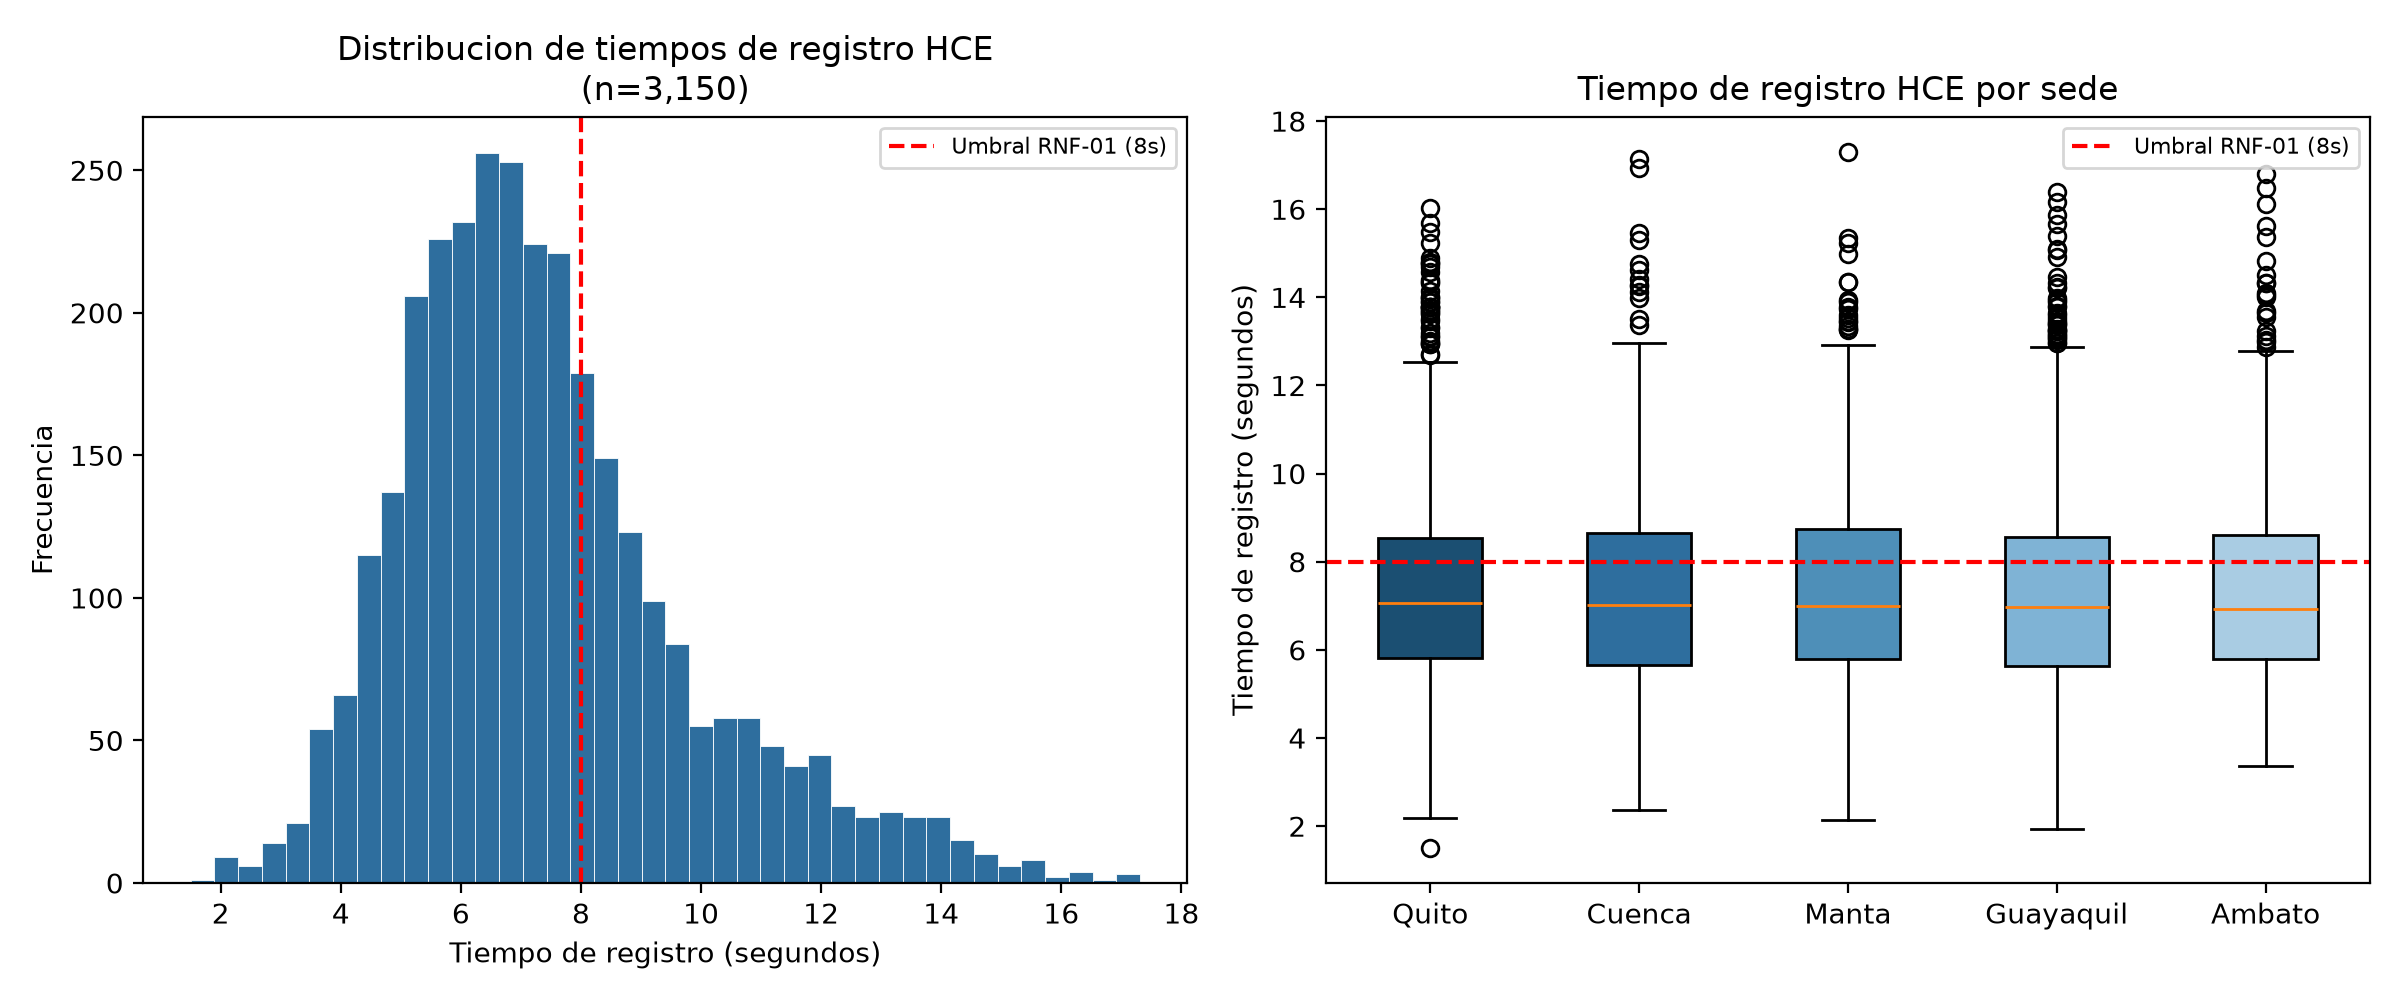
\includegraphics[width=\textwidth]{img/distribucion_tiempos_hce.png}
\caption{Izquierda: histograma de tiempos de registro (n=3\,150). La l\'inea roja indica el umbral RNF-01 (8s). Derecha: boxplot por sede, evidenciando consistencia entre sedes (Cobertura de Contexto).}
\end{figure}

\subsection{Impacto de las horas pico en la eficiencia}

\begin{figure}[H]
\centering
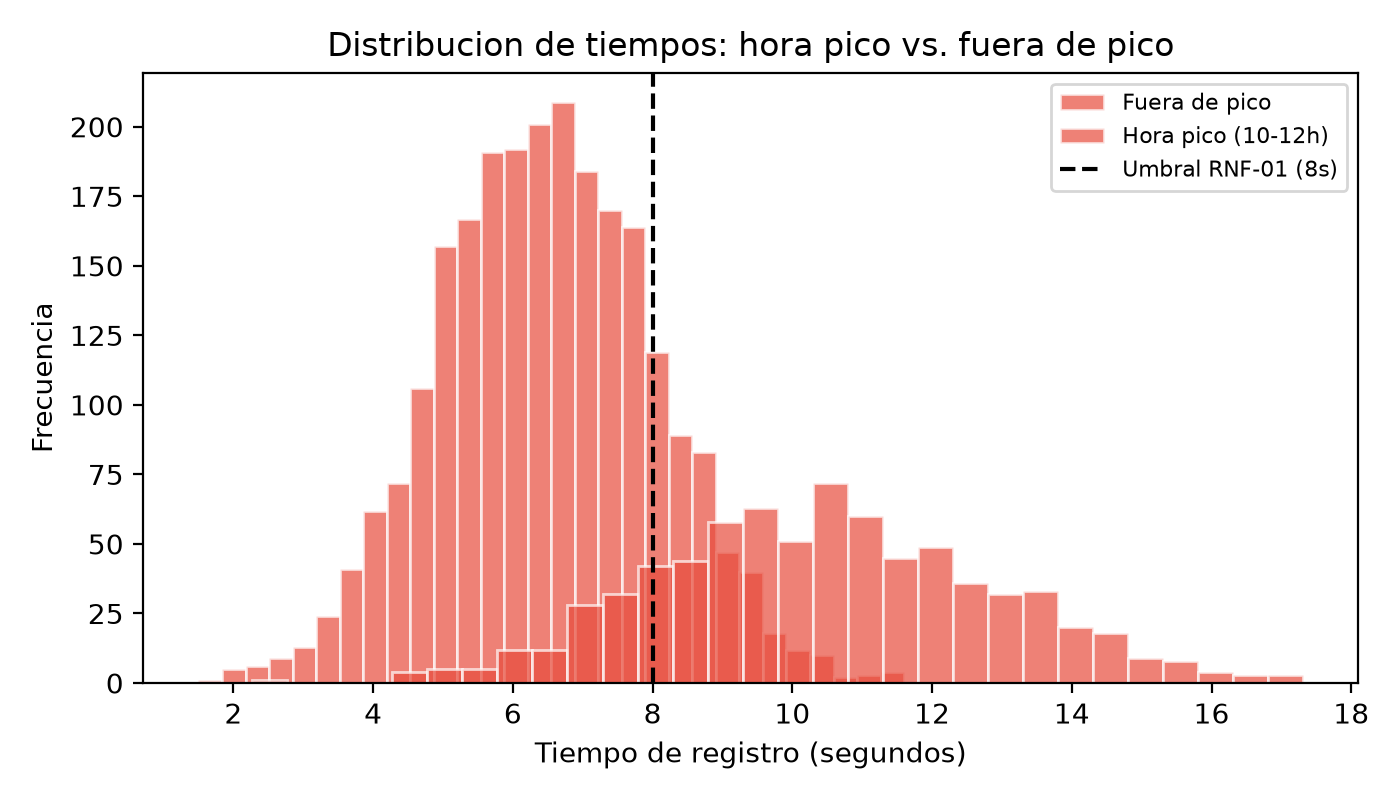
\includegraphics[width=0.8\textwidth]{img/pico_vs_no_pico.png}
\caption{Distribuci\'on de tiempos de registro: hora pico (10--12h, rojo) vs. fuera de pico (azul). Se observa un desplazamiento claro hacia tiempos mayores durante las horas de m\'axima carga, consistente con los hallazgos del Escenario 3.}
\end{figure}

\subsection{Efectividad por sede}

\begin{figure}[H]
\centering
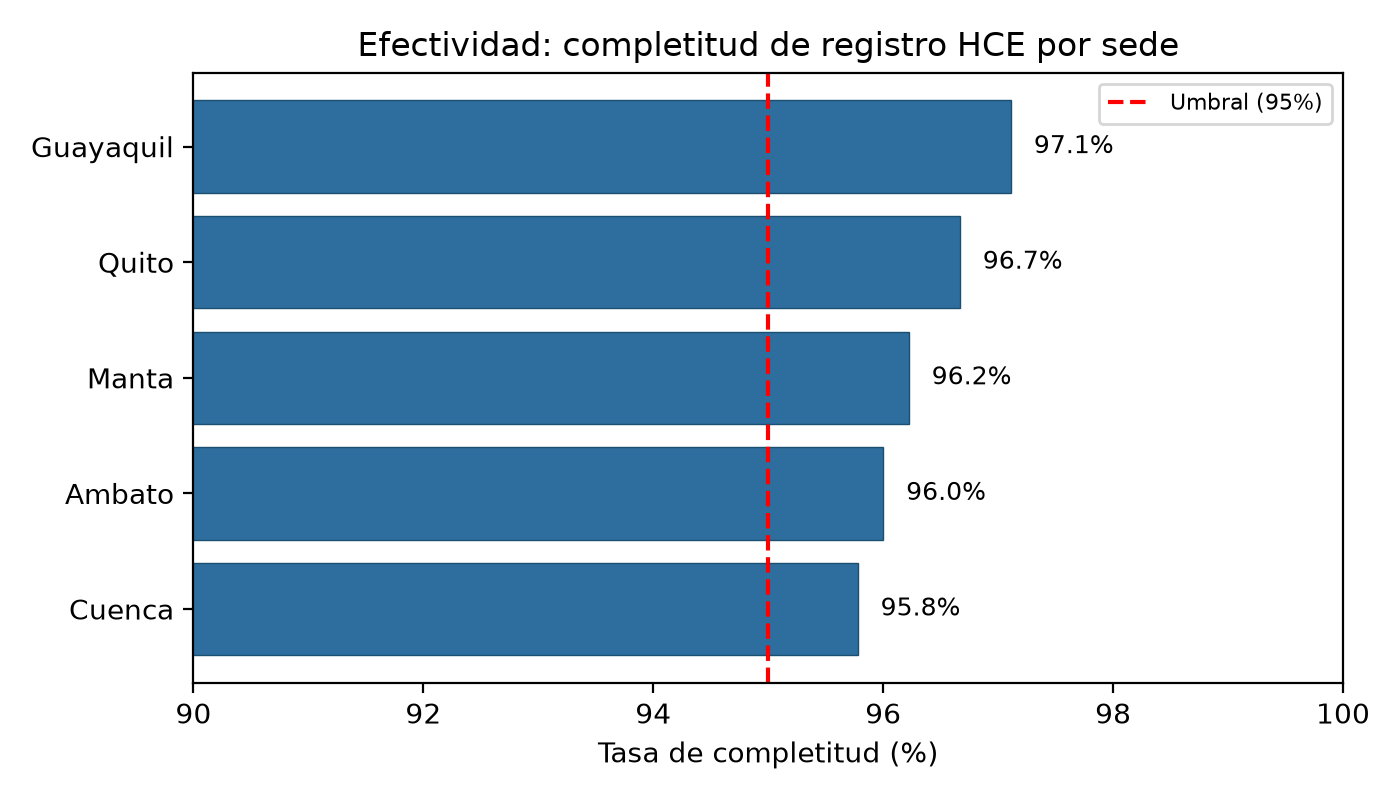
\includegraphics[width=0.8\textwidth]{img/efectividad_por_sede.png}
\caption{Tasa de completitud de registro HCE por sede. La l\'inea roja indica el umbral de 95\%. Todas las sedes superan el umbral, indicando que la Efectividad global cumple el objetivo.}
\end{figure}

\subsection{Encuestas de satisfacci\'on CSAT}

\begin{figure}[H]
\centering
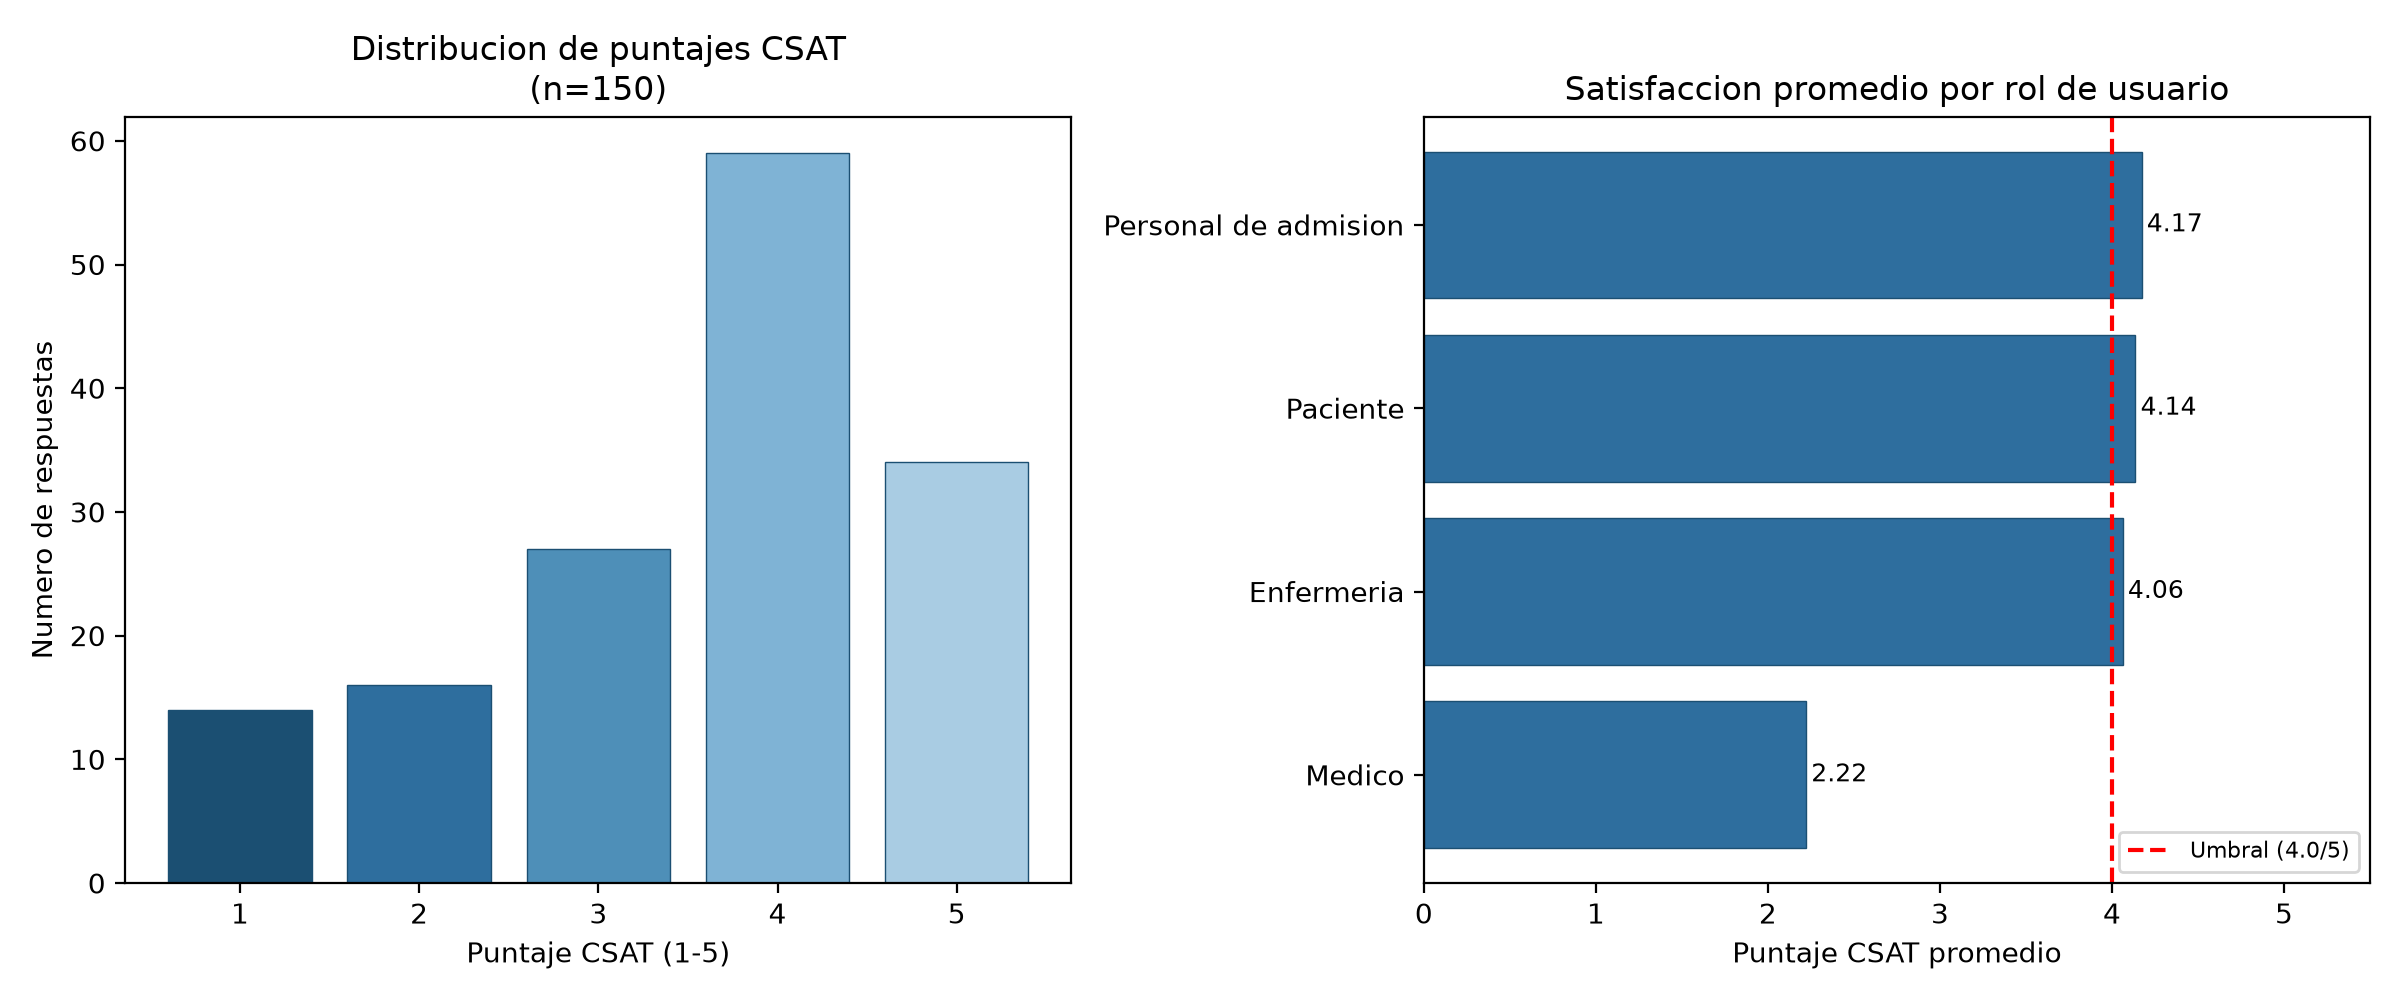
\includegraphics[width=\textwidth]{img/encuesta_csat.png}
\caption{Izquierda: distribuci\'on de puntajes CSAT (n=150). Derecha: promedio CSAT por rol de usuario. Los m\'edicos presentan la satisfacci\'on m\'as baja (2.22/5), consistente con la frustraci\'on por la lentitud del m\'odulo HCE documentada en el Escenario 3.}
\end{figure}

% ============================================================
\section{Preguntas de Discusi\'on}

\begin{enumerate}
    \item \textbf{?`Qu\'e riesgos introduce el uso de datos sint\'eticos en un programa de medici\'on de calidad en uso?}

    Los datos sint\'eticos pueden no reflejar patrones reales como estacionalidad, correlaciones entre m\'odulos, o eventos at\'ipicos (ca\'idas de red, actualizaciones de sistema). El principal riesgo es la \textbf{sobreconfianza}: si los datos sint\'eticos se ajustan demasiado bien a los umbrales, el equipo podr\'ia creer que el sistema cumple cuando en realidad no ha sido validado con datos de producci\'on. Por ello, los datos sint\'eticos deben usarse exclusivamente para \textbf{validar el pipeline de medici\'on} y nunca para tomar decisiones operativas.

    \item \textbf{?`Por qu\'e el sesgo intencional en las encuestas CSAT (m\'edicos con puntajes bajos) es \'util para validar el pipeline?}

    Porque refleja un patr\'on real observable en el caso MediSalud: los m\'edicos son los usuarios m\'as afectados por la lentitud del m\'odulo HCE (22.1 segundos promedio vs. 8 segundos de umbral). Si los datos sint\'eticos fueran uniformes, el pipeline no podr\'ia demostrar su capacidad de detectar diferencias significativas entre roles, que es precisamente uno de los hallazgos que la gerencia necesita para priorizar inversiones.

    \item \textbf{?`Qu\'e verificaci\'on adicional ser\'ia necesaria con datos de producci\'on?}

    Con datos reales, se deber\'ian a\~nadir: (a) verificaci\'on de integridad referencial entre tablas (e.g., que cada \texttt{medico\_id} en los logs exista en el directorio de personal), (b) detecci\'on de valores at\'ipicos (\textit{outliers}) mediante criterios estad\'isticos (e.g., IQR o z-score), (c) verificaci\'on de completitud temporal (que no haya d\'ias o franjas horarias sin registros, lo que podr\'ia indicar fallos de instrumentaci\'on), y (d) validaci\'on de consistencia cruzada entre fuentes (e.g., que el n\'umero de notas en logs coincida con el conteo en la base de datos de HCE).
\end{enumerate}

% ============================================================
\section{Conclusiones}

\begin{tcolorbox}[colback=green!5, colframe=green!50!black, title=Resultado obtenido]
\begin{itemize}
    \item Se generaron \textbf{tres conjuntos de datos base} (3\,150 logs de HCE, 150 encuestas CSAT, 3\,000 incidentes) que cubren las cinco m\'etricas del cat\'alogo ISO/IEC 25022 dise\~nado en el Escenario 6.
    \item Se valid\'o la \textbf{integridad de los datos} (0 nulos, 0 duplicados, 0 valores fuera de rango), estableciendo un protocolo de validaci\'on reproducible para cuando se integren datos de producci\'on.
    \item El an\'alisis exploratorio confirm\'o emp\'iricamente los patrones esperados: degradaci\'on en horas pico, baja satisfacci\'on de m\'edicos, y consistencia entre sedes, proporcionando las bases para la automatizaci\'on del Escenario 8.
\end{itemize}
\end{tcolorbox}

\end{document}
